\chapter{設計指標の構築}
\label{chap:designindex}

収穫対象の周辺には茎や葉が存在し, それによって果実や花柄の一部が隠れている場合がある. 
例えば \figref{Fig:plantex}のような場合において, 赤丸で示したピーマンは花柄が露出しているが果実は葉で隠れてしまっているのに対し, オレンジの丸で示したピーマンは花柄が葉で隠れているが果実は露出している.
赤丸で示されたピーマンは花柄にアプローチしやすく, AGRISTの「L」に搭載されている花柄に直接アプローチするタイプのエンドエフェクタが適していると考えられる.
一方でオレンジの丸で示されたピーマンは果実にアプローチしたほうがよく, 果実を掴んで引っ張るなどの方法で収穫するエンドエフェクタが良いのではないかと予想できる.
このように, どのエンドエフェクタが望まれるかは収穫対象の特性に依存しており, 設計に資する特性を数値化することは設計において有益である.
収穫物は多種多様であり, 一般論で議論することは難しいため,以後の議論はピーマンを対象に行う.

\vspace{5mm}
\begin{figure}[H]
     \centering
     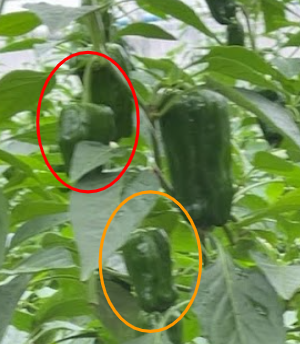
\includegraphics[width=100mm]{images/png/plantex.png}
     \caption{Example of green pepper crop}
     \label{Fig:plantex}
\end{figure}

%
\section{設計に資する収穫物の特性}
収穫物のどの部分に接近しやすいかで好ましいエンドエフェクタの形状が決まるため, 個体の特性よりも株の特性から議論する.
アプローチの容易さを推測する特性としては以下が考えられる.

\begin{center}
\begin{tabular}{|lr|} \hline
  花柄露出面積 & 露出している花柄の投影面積\\ \hline
  花柄側面障害物距離 & 花柄の横方向にある障害物の距離\\ \hline
  果実露出面積 & 露出している果実の投影面積\\ \hline
  果実側面障害物距離 & 果実の横方向にある障害物の距離\\ \hline
  果実上面障害物距離 & 果実の上方向にある障害物の距離\\ \hline
  果実下面障害物距離 & 果実の下方向にある障害物の距離\\ \hline
\end{tabular}
\end{center}
%
\section{エンドエフェクタの形状}
3.1節を踏まえて, アプローチの容易さを推測するために必要なエンドエフェクタの形状は以下が考えられる.

\begin{itemize}
  \item 花柄アプローチ幅: 花柄にアプローチする部分の幅
  \item 花柄アプローチ高さ: 花柄に触れる部分の高さ
  \item 花柄アプローチ面積: 把持または切断時に予想されるアプローチ部分の面積, (花柄アプローチ部分の高さ) \verb|×| (花柄の幅の平均)で算出する
  \item 果実アプローチ幅: 果実にアプローチする部分の幅, 幅の方向はエンドエフェクタによって異なる
  \item 果実アプローチ高さ: 果実に触れる部分の高さ
  \item 果実アプローチ面積: 把持時に予想されるアプローチ部分の面積, (果実アプローチ部分の高さ) \verb|×| (果実の幅の平均)で算出する
\end{itemize}
% \begin{center}
%   \begin{tabular}{|lr|} \hline
%     花柄アプローチ幅 & 花柄にアプローチする際の幅\\ \hline
%     花柄アプローチ高さ & 花柄に触れる部分の高さ\\ \hline
%     花柄アプローチ面積 & 花柄アプローチ部分の高さ * 花柄の幅\\ \hline 
%     果実アプローチ幅 & 果実にアプローチする際の幅\\ \hline
%     果実アプローチ高さ & 果実に触れる部分の高さ\\ \hline
%     果実アプローチ面積 & 果実アプローチ部分の高さ * 果実の幅\\ \hline 
%   \end{tabular}
%   \end{center}
%
\section{設計指標}
収穫物の特性とエンドエフェクタの形状から設計指標を構築する.
設計指標は以下のように設定した.

\begin{itemize}
  \item 花柄側面障害物間距離が許容範囲内か: $d_p$ \verb|>| $l_p$
  \item 花柄アプローチ面積より花柄が露出しているか: $S_p$ \verb|>| $S_papproach$
  \item 果実側面障害物間距離が許容範囲内か: $d_fside$ \verb|>| $l_fside$
  \item 果実上面障害物間距離が許容範囲内か: $d_fabove$ \verb|>| $l_fabove$
  \item 果実下面障害物間距離が許容範囲内か: $d_funder$ \verb|>| $l_funder$
  \item 果実アプローチ面積より果実が露出しているか: $S_f$ \verb|>| $S_fapproach$
\end{itemize}
%
\section{成功率の算出}
各エンドエフェクタはそれぞれピーマンにアプローチする部分が異なるため, 必要に応じて指標を取り入れることになる.
例えば, AGRISTのLに搭載されているエンドエフェクタの場合は, 果実にアプローチを行わないため, 花柄に関わる指標しか取り入れないこととなる.
取り入れた指標をすべて満たすものを成功とし, それ以外は失敗とする.
成功率$p_h$は以下のように表す.

\vspace{10mm}
成功率$p_h$ = 指標をすべて満たすもの / 計測した収穫物の数
\vspace{10mm}

AGRISTのLに搭載されているエンドエフェクタの場合, 成功率に関わる設計指標は, 花柄側面障害物間距離が許容範囲内かというのと花柄アプローチ面積よりも花柄が露出しているかの2つである.
よって成功率は以下のようになる.

\vspace{10mm}
$p_h = p(d_p > l_p \cap S_p > S_papproach)$
\vspace{10mm}

%